% !TeX spellcheck = ru_RU_yo
% !TEX program = xelatex

\documentclass[pta]{../../scs-iam}

\begin{document}

\newgeometry{
  top=20mm,
  right=15mm,
  bottom=20mm,
  left=20mm,
  bindingoffset=0cm
}

\thispagestyle{empty}

\begin{center}
  {
    \bfseries
    {
      \subnormal
      Министерство образования и науки Российской Федерации
    } \\[-0.5em]
    {
      \scriptsize
      ФЕДЕРАЛЬНОЕ ГОСУДАРСТВЕННОЕ АВТОНОМНОЕ ОБРАЗОВАТЕЛЬНОЕ УЧРЕЖДЕНИЕ ВЫСШЕГО ОБРАЗОВАНИЯ
    } \\[-0.25em]
    {
      \subnormal
      “САНКТ-ПЕТЕРБУРГСКИЙ НАЦИОНАЛЬНЫЙ ИССЛЕДОВАТЕЛЬСКИЙ \\[-0.5em]
      УНИВЕРСИТЕТ ИНФОРМАЦИОННЫХ ТЕХНОЛОГИЙ, \\[-0.75em]
      МЕХАНИКИ И ОПТИКИ”
    }
  }
\end{center}

\small

\begin{center}
  \vskip -1.5em
  {
    \bfseries
    {
      \large
      ОТЗЫВ РУКОВОДИТЕЛЯ \\
    }
    О  ВЫПУСКНОЙ  КВАЛИФИКАЦИОННОЙ  РАБОТЕ
  }
\end{center}

\vskip -1.25em

{
  \parindent0pt
  
  \textbf{Студент}
  \underline{\text{\strut Кузнецов А.А.~\,}}
  \hfill
  \textbf{Группа}
  \underline{\text{\strut P4215~\,}}
  \hfill
  \textbf{Кафедра}
  \underline{\text{\strut ИПМ~\,}}
  \hfill
  \textbf{Факультет}
  \underline{\text{\strut ПИиКТ~\,}} \\[-1.25em]
  
  \titledline{\textbf{Квалификация}}
  \uline{магистр\hfill} \\[-1.5em]

  \titledline{\textbf{Направление подготовки (специальность)}}
  \uline{09.04.01 -- Информатика и вычислительная техника\hfill} \\[-1.5em]

  \titledline{\textbf{Направленность (профиль)}}
  \uline{09.04.01 -- Математические модели и компьютерное моделирование\hfill} \\[-1.5em]

  \titledline{\textbf{Наименование темы}}
  \uline{Разработка веб-приложения для работы с программным пакетом высоко\-точного позиционирования RTKLIB\hfill} \\[-1.5em]

  \titledline{\textbf{Рецензент}}
  $\underset{
    \text{\scriptsize (Фамилия, И., О., место  работы, должность, ученое звание, степень)}
  }{
    \underline{\makebox[\remaining][l]{Соснин В.В., к.т.н., доцент}}
  }$ \\[-2.5em]
}

\begin{center}
  \textbf{ПОКАЗАТЕЛИ ОЦЕНКИ ВЫПУСКНОЙ КВАЛИФИКАЦИОННОЙ РАБОТЫ}
\end{center}

\vskip -1.75em

{
  \parindent0pt
  \footnotesize
  
  \begin{figure}[h!]
    \centering
    \setlength{\fboxsep}{0pt}
    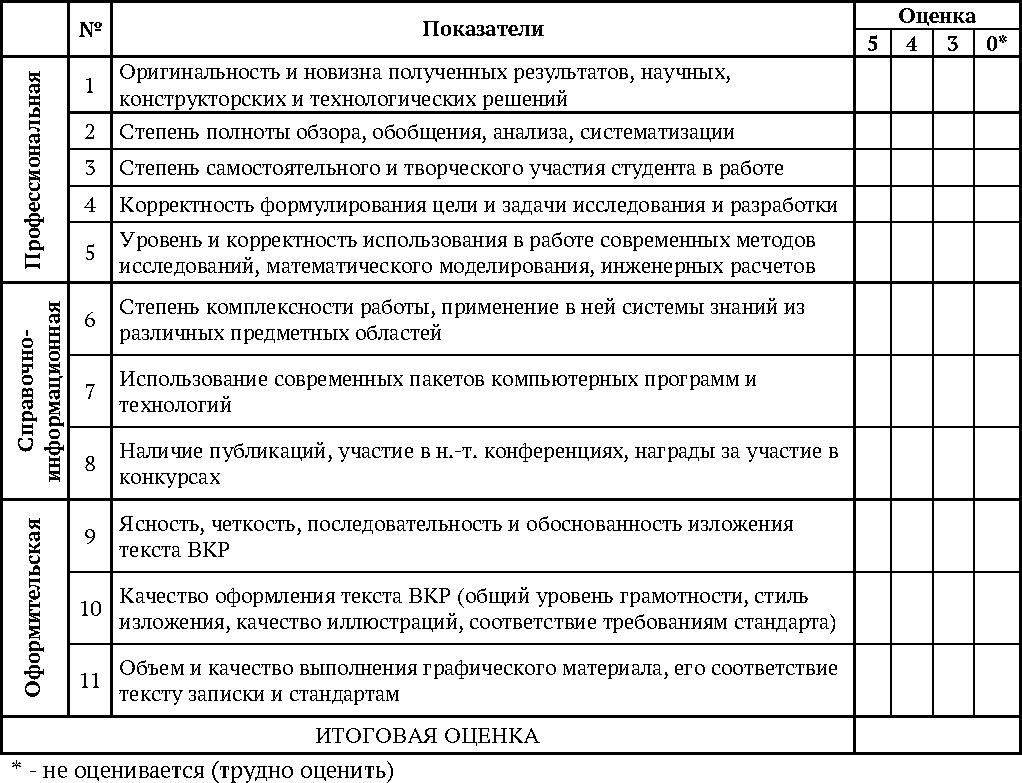
\includegraphics[width=\textwidth]{table}
  \end{figure}
}

\clearpage

\newgeometry{
  top=20mm,
  right=20mm,
  bottom=20mm,
  left=15mm,
  bindingoffset=0cm
}

\thispagestyle{empty}

{
  \parindent 0pt

  \textbf{Отмеченные достоинства:} \\
  \uline{
    1. Проведён качественный обзор проблем и решений, существующих в области высокоточного позиционирования. \hfill
  } \\
  \uline{
    2. Подробна описана созданная в рамках выполнения работы архитектура разрабатываемого при\-ложения. \hfill
  } \\
  \uline{
    3. Работа содержит подробное описание всех этапов проектирования, разработки и апробации разрабатываемого решения. \hfill
  } \\[-1em]

  \textbf{Отмеченные недостатки:} \\
  \uline{
    1. Отсутствует описание шаблона проектирования, использованного при разработке JavaScript\-приложения. \hfill
  } \\
  \uline{
    2. Отсутствие определений специфических для геодезии терминов усложняет восприятие работы. \hfill
  } \\[-1em]
  
  \textbf{Заключение:}
  Считаю, что ВКР студента Кузнецова А.А. на тему: <<Разработка веб-приложения для работы с программным пакетом высокоточного позиционирования RTKLIB>> соответствует требованиям Университета ИТМО, предъявляемым к ВКР, и заслуживает оценки <<отлично>>, а её автор -- присуждения квалификации магистр по направлению подготовки (специальности) 09.04.01. \\
  
  Руководитель ВКР~
  \signature~
  $\underset{
    \text{\scriptsize (Фамилия, И., О.)}
  }{
    \underline{\makebox[7em][s]{\strut\hfill Соснин В.В.~\hfill}}
  }$
  \hfill
  \specialdatetemplate \\
  
  С отзывом ознакомлен~
  \signature~
  $\underset{
    \text{\scriptsize (Фамилия, И., О.)}
  }{
    \underline{\makebox[7em][s]{\hfill Кузнецов А.А.\hfill}}
  }$
  \hfill
  \specialdatetemplate \\
  
  Принято~
  \specialdatetemplate
  \hfill
  Секретарь ГЭК~
  \signature~
  $\underset{
    \text{\scriptsize (Фамилия, И., О.)}
  }{
    \underline{\makebox[6em][s]{\strut}}
  }$
}

\end{document}
